% Template for Elsevier CRC journal article
% version 1.2 dated 09 May 2011

% This file (c) 2009-2011 Elsevier Ltd.  Modifications may be freely made,
% provided the edited file is saved under a different name

% This file contains modifications for Transportation Research Procedia

% Changes since version 1.1
% - added "procedia" option compliant with ecrc.sty version 1.2a
%   (makes the layout approximately the same as the Word CRC template)
% - added example for generating copyright line in abstract

%-----------------------------------------------------------------------------------

%% This template uses the elsarticle.cls document class and the extension package ecrc.sty
%% For full documentation on usage of elsarticle.cls, consult the documentation "elsdoc.pdf"
%% Further resources available at http://www.elsevier.com/latex

%-----------------------------------------------------------------------------------

%%%%%%%%%%%%%%%%%%%%%%%%%%%%%%%%%%%%%%%%%%%%%%%%%%%%%%%%%%%%%%
%%%%%%%%%%%%%%%%%%%%%%%%%%%%%%%%%%%%%%%%%%%%%%%%%%%%%%%%%%%%%%
%%                                                          %%
%% Important note on usage                                  %%
%% -----------------------                                  %%
%% This file should normally be compiled with PDFLaTeX      %%
%% Using standard LaTeX should work but may produce clashes %%
%%                                                          %%
%%%%%%%%%%%%%%%%%%%%%%%%%%%%%%%%%%%%%%%%%%%%%%%%%%%%%%%%%%%%%%
%%%%%%%%%%%%%%%%%%%%%%%%%%%%%%%%%%%%%%%%%%%%%%%%%%%%%%%%%%%%%%

%% The '3p' and 'times' class options of elsarticle are used for Elsevier CRC
%% The 'procedia' option causes ecrc to approximate to the Word template
\documentclass[5p,times,procedia]{elsarticle}
\flushbottom

%% The `ecrc' package must be called to make the CRC functionality available
\usepackage{ecrc}
\usepackage{amsmath}
\usepackage[utf8]{inputenc}
\usepackage[mode=buildnew]{standalone}% requires -shell-escape
\usepackage{tikz}
\usepackage{pgfplots}
\usepgfplotslibrary{groupplots}
\usepgfplotslibrary{dateplot}
\pgfplotsset{compat=newest}

%% The ecrc package defines commands needed for running heads and logos.
%% For running heads, you can set the journal name, the volume, the starting page and the authors

%% set the volume if you know. Otherwise `00'
\volume{00}

%% set the starting page if not 1
\firstpage{1}

%% Give the name of the journal
\journalname{Procedia CIRP}

%% Give the author list to appear in the running head
%% Example \runauth{C.V. Radhakrishnan et al.}
\runauth{Author name}

%% The choice of journal logo is determined by the \jid and \jnltitlelogo commands.
%% A user-supplied logo with the name <\jid>logo.pdf will be inserted if present.
%% e.g. if \jid{yspmi} the system will look for a file yspmilogo.pdf
%% Otherwise the content of \jnltitlelogo will be set between horizontal lines as a default logo

%% Give the abbreviation of the Journal.
\jid{trpro}

%% Give a short journal name for the dummy logo (if needed)
%\jnltitlelogo{Transportation Research}

%% Hereafter the template follows `elsarticle'.
%% For more details see the existing template files elsarticle-template-harv.tex and elsarticle-template-num.tex.

%% Elsevier CRC generally uses a numbered reference style
%% For this, the conventions of elsarticle-template-num.tex should be followed (included below)
%% If using BibTeX, use the style file elsarticle-num.bst

%% End of ecrc-specific commands
%%%%%%%%%%%%%%%%%%%%%%%%%%%%%%%%%%%%%%%%%%%%%%%%%%%%%%%%%%%%%%%%%%%%%%%%%%

%% The amssymb package provides various useful mathematical symbols

\usepackage{amssymb}
%% The amsthm package provides extended theorem environments
%% \usepackage{amsthm}

%% The lineno packages adds line numbers. Start line numbering with
%% \begin{linenumbers}, end it with \end{linenumbers}. Or switch it on
%% for the whole article with \linenumbers after \end{frontmatter}.
%% \usepackage{lineno}

%% natbib.sty is loaded by default. However, natbib options can be
%% provided with \biboptions{...} command. Following options are
%% valid:

%%   round  -  round parentheses are used (default)
%%   square -  square brackets are used   [option]
%%   curly  -  curly braces are used      {option}
%%   angle  -  angle brackets are used    <option>
%%   semicolon  -  multiple citations separated by semi-colon
%%   colon  - same as semicolon, an earlier confusion
%%   comma  -  separated by comma
%%   numbers-  selects numerical citations
%%   super  -  numerical citations as superscripts
%%   sort   -  sorts multiple citations according to order in ref. list
%%   sort&compress   -  like sort, but also compresses numerical citations
%%   compress - compresses without sorting
%%
%\biboptions{authoryear}

% \biboptions{}

% if you have landscape tables
\usepackage[figuresright]{rotating}
%\usepackage{harvard}
% put your own definitions here:x
%   \newcommand{\cZ}{\cal{Z}}
%   \newtheorem{def}{Definition}[section]
%   ...

% add words to TeX's hyphenation exception list
%\hyphenation{author another created financial paper re-commend-ed Post-Script}

% declarations for front matter

\usepackage[bookmarks=false]{hyperref}
    \hypersetup{colorlinks,
      linkcolor=blue,
      citecolor=blue,
      urlcolor=blue}
\usepackage{xcolor}
\newcommand{\AP}[1]{{\color{blue} {\bf (AP: #1)}}}
\newcommand{\LS}[1]{{\color{purple} {\bf (LS: #1)}}}
\newcommand{\MW}[1]{{\color{teal} {\bf (MW: #1)}}}
\newcommand{\JG}[1]{{\color{green} {\bf (JG: #1)}}}
\newcommand{\DSt}[1]{{\color{orange} {\bf (DSt: #1)}}}

\begin{document}
\begin{frontmatter}

%% Title, authors and addresses

%% use the tnoteref command within \title for footnotes;
%% use the tnotetext command for the associated footnote;
%% use the fnref command within \author or \address for footnotes;
%% use the fntext command for the associated footnote;
%% use the corref command within \author for corresponding author footnotes;
%% use the cortext command for the associated footnote;
%% use the ead command for the email address,
%% and the form \ead[url] for the home page:
%%
%% \title{Title\tnoteref{label1}}
%% \tnotetext[label1]{}
%% \author{Name\corref{cor1}\fnref{label2}}
%% \ead{email address}
%% \ead[url]{home page}
%% \fntext[label2]{}
%% \cortext[cor1]{}
%% \address{Address\fnref{label3}}
%% \fntext[label3]{}

\dochead{54th CIRP Conference on Manufacturing Systems}%

\title{Predictive analytics in quality assurance for assembly processes:
       lessons learned from a case study at an industry 4.0 demonstration cell}

%% use optional labels to link authors explicitly to addresses:
%% \author[label1,label2]{<author name>}
%% \address[label1]{<address>}
%% \address[label2]{<address>}



\author[a]{Peter Burggräf}
\author[a]{Johannes Wagner}
\author[a]{Benjamin Koke}
\author[a]{Fabian Steinberg} 
\author[a]{Alejandro R. Pérez M.}
\author[a]{Lennart Schmallenbach}
\author[b,c]{Jochen Garcke}
\author[b]{Daniela Steffes-lai}
\author[b,d]{Moritz Wolter}

%\ead{author@institute.xxx}

\address[a]{Chair of International Production Engineering and Management (IPEM), Universität Siegen, Paul-Bonatz-Straße 9-11, Siegen - 57076, Germany}
\address[b]{Fraunhofer Institute for Algorithms and Scientific Computing (SCAI), Schloss Birlinghoven 1, Sankt Augustin- 53757, Germany}
\address[c]{Institut for Numerical Simulation, Universität Bonn, Endenicher Allee 19b, 53115 Bonn}
\address[d]{Institut for Computer Science, Universität Bonn, Endenicher Allee 19a, 53115 Bonn}

\aucores{* Corresponding author. Tel.: +49-271-740-4509; fax: +49-271-740-2630. {\it E-mail address:} alejandro.perez@uni-siegen.de}

\begin{abstract}
%% Text of abstract
Quality assurance (QA) is an important task in manufacturing to assess whether products 
meet their specifications. However, QA might be expensive, time-consuming, incomplete, or delayed.
This paper presents a solution for predictive analytics in QA based on machine sensor values during
production while employing machine-learning models based on logistic regression in a controlled environment. 
Furthermore, we present lessons learned while implementing this model, which helps to reduce complexity in
further industrial applications. The paper’s outcome proves that the developed model was able to predict
product quality, as well as to identify the correlation between machine-status and faulty product occurrence.
\end{abstract}

\begin{keyword}
Machine-Learning \sep Predictive Quality \sep Production \sep Quality Assurance \sep Logistic Regression 

%% keywords here, in the form: keyword \sep keyword

%% PACS codes here, in the form: \PACS code \sep code

%% MSC codes here, in the form: \MSC code \sep code
%% or \MSC[2008] code \sep code (2000 is the default)

\end{keyword}
%\cortext[cor1]{Corresponding author. Tel.: +0-000-000-0000 ; fax: +0-000-000-0000.}

\end{frontmatter}


\section{Introduction} % 1 Page (incl authors, abstract)

\AP{\begin{itemize}
       \item	Products’ quality must always be guaranteed.
       \item	In certain cases (especially in series assembly production) there is a delay between quality inspection
              and end of the production process high potential for producing scrap 
       \item	By doing quality inspection based on samples, there is still a risk of sending NOK parts to customers
       \item	The cost of quality checks might be expensive
       \item	Quality assurance is normally done at the end of production (for assembly processes)   
       \item	Early prediction of the production’s quality  would help to decrease the amount of scrap  and the risk of sending NOK parts to customers
       \item	Variable predictions by using machine learning models is currently widely used in diverse fields due to its accurate predictions with the data collected from the machines, 
              prediction models can be implemented for specific predicted values
\end{itemize}}

\section{Related Works} % 1 Page \Lennart

\subsection{Quality check in production} % Basic books (find summarize) basic concepts

The quality control of production processes and products is one part of the general quality management
and contains the measures and activities needed to fulfill the quality requirements \cite{illes2017new}.
According to Illés, currently there are three established tools and methods of quality control \cite{illes2017new}:
The Statistical Process Control (SPC), Auditing and Total Quality Control (TQC).   
The SPC is used to monitor the production process using recorded data values for the quality characteristics and to indicate any significant changes
in the quality characteristics in the production process \cite{selvamuthu2018introduction}. It can take place before and after a manufacturing process
as off-line SPC or implemented in the manufacturing process as in-line SPC.
With SPC, large batches can be checked, but it is only possible, if the variance of the process and product parameters is small enough,
to ensure process capability \cite{kahle2013zuverlaessigkeitsanalyse}.
Auditing, in this case especially product and process auditing, is the most fundamental quality control technique. 
Product and process auditing is the independent examination of product and process quality to provide information. This is executed by
an independent auditor, based on sampling, or checking records. But the auditor is just reporting incorrect processes or products. The required adapting is done by others \cite{fox1993quality}.
Both statistical methods and hundred percent controls can be applied as an audit tool.
Statistical methods such as acceptance sampling or quality control charts represent a compromise between zero and hundred percent control \cite{selvamuthu2018introduction, kurniati2015quality}.
While the SPC mostly optimizes the capability of the process, for example the acceptance plan prevents the nonconforming product to be pass and then delivered to the next process or the customer \cite{kurniati2015quality}.
In the case of a hundred percent control, this is associated with higher costs and a higher requirement of time, compared to a quality control based on a machine learning model.
Statistical methods are faster as hundred percent controls, but have the same problem like the SPC: Because they are based on assumptions, this methods are prone to errors,
if the variance of the product quality is to high.
The concept of TQC is to extend the scope of quality control to the whole company and product life cycle,
by involving all departments of the organization \cite{illes2017new}.
The quality characteristics of a product can be classified as variables or attributes.
Variables are measurable characteristics, which are shown as numbers. On the contrary,
attributes are not measureable and can only take the value go or no-go \cite{mitra2016fundamentals}. 
The advantage of variable measurements is that in the event of a defective intermediate or end product, 
precise measured values are available, which enable precise adjustment of the process parameters. 
This allows the desired quality to be restored. With that in mind, a predictive quality control is a promising solution.

\AP{
\begin{itemize}
\item How quality check is done in production
\item Concepts and sampling plan
\item Attributive vs Variable measurements [VM has higher measurement accuracy, reason why it’s better to use regression model]
\end{itemize}}

\subsection{Predictive analytics in production}

Predictive analytics discover according to Delen and Damirkan explanatory and predictive patterns which represents 
the inherent relationships between data inputs and outputs, using data and mathematical techniques \cite{delen2013data}. 
This offers a wide range of applications. In the context of industrial or production enviroments, this includes in the areas of Processes, Products and Machines and Assets for example 
predictive maintenance, product design or optimization of routing and scheduling \cite{krauss2019machine}. 
Predictive analytics combined with quality control can be a powerful tool, because it is an improvement compared with the mentioned earlier currently
etablished quality control methods, in terms of speed, accuracy and time delay.
So far, only in exceptional cases in the literature is a combination of predictive analytics and quality control found \cite{aumi2012model, ritter1992neue}. With regard to general approaches to the use of predictive analytics,
for example in the form of machine learning in quality prediction, there is a lack in the literature. 
Related work, e.g from Krauß focused on automated machine learning for predictive quality in production \cite{krauss2020automated} and a product quality prediction in a process chain \cite{krauss2019machine}. 
The few existing approaches are extended by this paper in that a demonstrator executes an industry-unspecific production/assembly process,
the collection and processing of the data from the process parameters in continous and a few different ML algorithms are used for prediction, 
in order to determine, which algorithms are most advantageous for predicting the quality of an outcoming product. 
In addition, it is described in detail how the collected data was collected, prepared and processed.



\AP{
Predictive analytics as concepts. Implementation in production
\begin{itemize}
       \item Predictive Maintenance
       \item Scheduling
       \item Other
\end{itemize}       
If happens to be something with P.A. Quality Check
\begin{itemize}
       \item	Predictive analytics in production focusing in QA
       \item	Existing approaches and methods
\end{itemize}      
Note: Ideal is to find a gap in the literature, that proves why do we do it and why it is important
}


\section{The case industry 4.0 demonstration cell} % (taken from title) % 3/4 Page

In our work we applied a case-based research approach \cite{yin2017case} to answer the research question. 
One central motivation for a case-based research approach is to gain insights for real needs, rather than to develop theories without practical relevance \cite{cutcheon1993case}. %This sentence can be deleted if needed.
In addition case-based research approaches have already been successfully applied in the area of quality prediction based on process parameters (see, for example, ....). % @Lennart: hier müssen entsprechend Beispiele eingetragen werden
\AP{ 
       - How does the previous sentences apply to the democell?
       - This suits better in the methods section}

Our case of study is an abstraction of an assembly process at the industry. The industry 4.0 demonstration cell is composed by three independent conveyor belts, a robotic assembly arm, a laser scanner used for quality control as well as a wide range of sensors, all orchestrated by a SIEMENS PLC S7-1200. 
The assembly process done at this demostration cell consist on stacking two disk of different size on the top of each other. The quality of the pseudo products is later evaluated by the laser scanner by evaluating the concentricity of both disk. If the disk's concentricity is within a tolerance of 1.5mm, the piece is classified as OK, if not, it shall be classified as NOK.
By considering that malfunctions can occurs during real production processes at industries, our demonstration cell is able to simulate failures in diverse areas, such as:

\begin{itemize}
       \item Assemble errors due to robotic arm
       \item Bearing damage on the conveyor belt
       \item Resistance on the conveyor belt
       \item Leakage in the compressed air system
       \item Productivity limit reached
       \item Missing material
\end{itemize}

Those simulated failures have a real impact in the data collected by the sensors. Anomalies can be observed at the vibration sensors, temperature rise, fluctuations in the air pressure system, noticiable shifting on pieces' position as well as the stop of the process.

The continous data collection and clear correlation between the machine parameter is the ideal play-ground to implement a sandbox for machine learching implementations. With this in mind, our goal is to predict the quality of the product (concentricity of the assambled parts), prior to the actual quality check done by the laser scanner. The findings gained with the demonstration cell can be transferred to various real assembly processes and use cases, due to its manageable size and high degree of scalability. This would be an step forwards for future implementations at the industry, where the quality predictions might determine early enough, the next steps for the assambled pieces.


\begin{figure}
       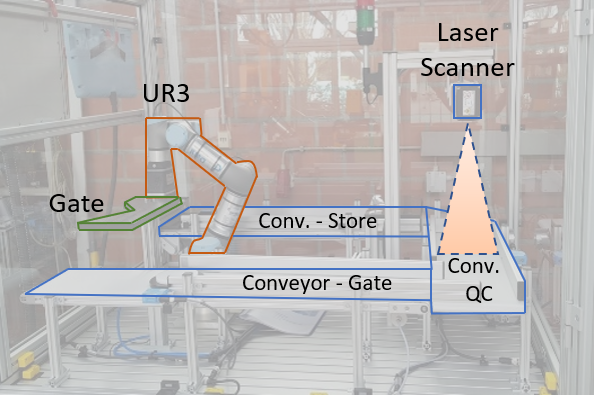
\includegraphics[width=.45\textwidth]{img/demozelle}
       \caption{The industry 4.0 demonstration cell at the University of Siegen}
\label{fig:ind_cell}
\end{figure}

\begin{figure}
       \includestandalone[width=.45\textwidth]{img/arm_data_plot}
       \caption{Robot arm movement patterns. We show the movement of the 
                cell's robot arm, its grippers and an encoding of the overall
                position in the system. The changes in the grip flag are triggered,
                when the gripper opens or closes. Zero indicates an open, while
                one indicates a closed gripper. The position flags marks the state
                of the cell's arm. 0 means the black disk is in store,
                one that the black disk is in the gate, two that the white disk
                is in store and three that the white disk is located in gate.
             }
\label{fig:robot_pos_cell}
\end{figure}

\AP{ @Moritz: Why is the figure 2 whithin the area of the Demozelle section?}

\section{Methods} %3/4 Page

Data  is collected from the demonstration cell and analyzed.

\subsection{Measurement}
\DSt{
- what is this section about?
}

\subsection{Machine Learning}
We compare Support Vector Machines (SVM), Multilinear Perceptrons
\cite{bishop2006pattern} as well as Random forests in the task of
quality prediction. 


\section{Experiments}

\subsection{Recording the data}
\DSt{
- could we include collection via OPCUA server? or manually? 
}

\subsection{Classifier optimization and testing}\label{sec:ml_exp}
The robot's position at disc drop is marked in 
Figure~\ref{fig:robot_pos_cell}. The quality prediction problem is 
framed as a classification task. The input vectors which we feed into our
classifiers consists of the arm positions at the disc drops for both
discs in three dimensions, as well as the largest recorded belt speed
of all three belts. The interpretation of the quality measurement is 
used as the training target. It can be good or bad which we encode as 
zero and one.

We work with a total of 132 measurements. Each containing arm and belt data
logs of individual cell runs. 20 samples are set aside at random for testing 
purposes, leaving 112 training samples. The random number generator seed is
set to one in order to ensure the train and test set splits are identical 
for all experiments.

We compare a total of three different classifier architectures on the data.
A Support Vector Machine (SVM), a multilinear perceptron and a Random Forest
structure. All three methods are trained using standard hyperparameters.
\footnote{In order to allow exact reproduction of these results source
code is available at \url{https://github.com/manubrain/Demo-Cell-Classification}}
\begin{table}
       \centering
       \begin{tabular}{ c c }
              Support Vector Machine & 95.\% \\
              Multilinear Perceptron & 95.\% \\
              Random Forest          & 100.\%
       \end{tabular}
       \caption{Method comparison for our annomaly detection task 
                using the industry demo data test set.}
       \label{tab:class_comp}
\end{table}
Results are shown in table~\ref{tab:class_comp}. For 55 of the total 132 samples
quality measurements indicate a problem. This sets the 
baseline over the entire data set, that would be obtained by simply labeling all samples
as good. Over the entire data set, we require to classify more than 58.3\% of the data correctly.
The test set contains eight incorrect samples. We would therefore expect any naive classifier
to produce a 60\% accuracy, which we have to beat. In Table~\ref{tab:class_comp},
we observe that this is indeed the case for all three approaches evaluated here.
The random forest performed best in this case.

\section{Conclusion}

\subsection{Lesson Learned} % 1/2 Page

\AP{explain experiences by doing the research

- Connection problem between devices
- Missing tags  
- Interpretation of data: preprocessing   
   - What data is relevant?
- Data sample size
- ML implementation @Moritz

}

\section{Conclusion} % 1/2 Page

\section*{Acknowledgments}
This project was partly supported by the german and european IKT.NRW
project "`ManuBrain"' 
\DSt{
do we need to include ManuBrain reference here?
}

\bibliographystyle{abbrv}
\bibliography{bib}

\end{document}
